\documentclass[12pt]{article}

\usepackage{se-alexandre}

\usepackage{graphicx,url}

\usepackage[brazil]{babel}   
\usepackage[utf8]{inputenc}  

     
\sloppy

\title{Trabalho da disciplina de Sistemas Evolutivos:\\ A Cellular Automata
 Model of Population Infected by Periodic Plague}

\author{Alexandre G. da Costa\inst{1}}


\address{Centro de Desenvolvimento Tecnológico -- Universidade Federal de
 Pelotas
  (UFPEL)\\
  Pelotas -- RS -- Brasil
  \email{alexandre.costa@inf.ufpel.edu.br}
}

\begin{document} 

% ----------------------------------------------------------------------------
\maketitle

% ----------------------------------------------------------------------------
\begin{abstract}
  This meta-paper describes the style to be used in articles and short papers
  for SBC conferences. For papers in English, you should add just an abstract
  while for the papers in Portuguese, we also ask for an abstract in
  Portuguese (``resumo''). In both cases, abstracts should not have more than
  10 lines and must be in the first page of the paper.
\end{abstract}
  
% ----------------------------------------------------------------------------   
\begin{resumo} 
  Este trabalho descreve a implementação do artigo proposto na disciplina de
  Sistemas Evolutivos e propõe uma nova abordagem da implementação. Esse
  artigo descreve um algoritmo que evolui.
\end{resumo}

% ----------------------------------------------------------------------------
\section{Introdução}

Automato celular é um modelo matemático que foi desenvolvido para simular a
evolução natural, por exemplo \textit{Game of Life}. Pois ele define tanto o
meio ambiante como também os indivíduos.


% ----------------------------------------------------------------------------
\section{Trabalhos Relacionados}
% Nesta sessão será explicado em detalhes o artigo referencial.

O artigo referencial abordado neste trabalho foi \textit{A Cellular Automata 
Model of Population Infected by Periodic Plague} de Witold Dzwinel. Nesse
artigo Dzwinel propõe um modelo complementar ao \textit{Penna paradigm}
\cite{almeida1998theoretical, de1998strategies} que considera a mutação
genética. Esse modelo complementar objetiva analisa a influência de fatores
ambientais sobre o processo de envelhecimento.

O modelo implementado no trabalho de \cite{dzwinel:04} assume que o conjunto
$S(t)$ de indivíduos é jogado aleatoriamente em uma matriz bi-dimensional
de um \textbf{Automato Celular} (AC). Cada indivíduo fica em uma célula e
carrega um código genético binário Figura \ref{fig:codigo-genetico} onde é
mostrado um código genético de oito bits de um indivíduo.

\begin{figure}[ht]
\centering
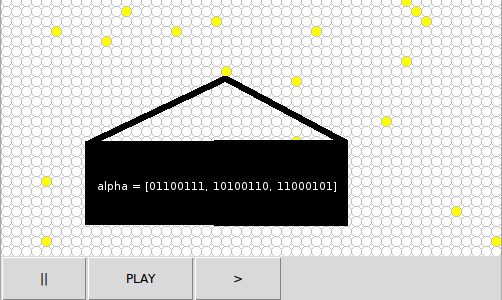
\includegraphics[width=.3\textwidth]{imagens/codigo-genetico}
\caption{Exemplo do código genético de um indivíduo.}
\label{fig:codigo-genetico}
\end{figure}

O código genético é composto de três vetores binários cada um corresponde a um
episódio de vida: a juventude ``\textbf{y}'', a maturidade ``\textbf{m}'' e a
velhice ``\textbf{o}''. Eles não representam a idade biológica dos indivíduos
da matriz, mas sim a capacidade de reprodução. Apenas indivíduos maduros podem
reproduzirem-se e ocorre quando esta sendo testado a vizinhança de Moore de
uma célula desocupada. Essa reprodução é baseada no operador de
\textit{cross-over} dos algoritmos genéticos.

O tempo de vida de um indivíduo é representado pelo número de 1's no código
genético. Já o tempo máximo de vida é o numero de 1's e 0's dentro do mesmo.
Cada ``1'' do código genético é lido a cada evolução quando o ultimo for lido
o indivíduo é removido da matriz CA.

$A = \left \{a_{ij}\right \}_{NxN}$ é uma matriz de possíveis localizações de
indivíduos na matriz do automato celular. A variável $a_{ij}$ é uma matriz
binária de NxN elementos. Quando $a_{ij} = 1$ a célula estará ocupada, já para
$a_{ij} = 0$ a célula não estará ocupada. Um indivíduo é definido pela matriz
$\alpha _{ij}$, a Figura \ref{fig:estrutura-alpha} mostra a estrutura da
matriz alpha.

\begin{figure}[h!]
\centering
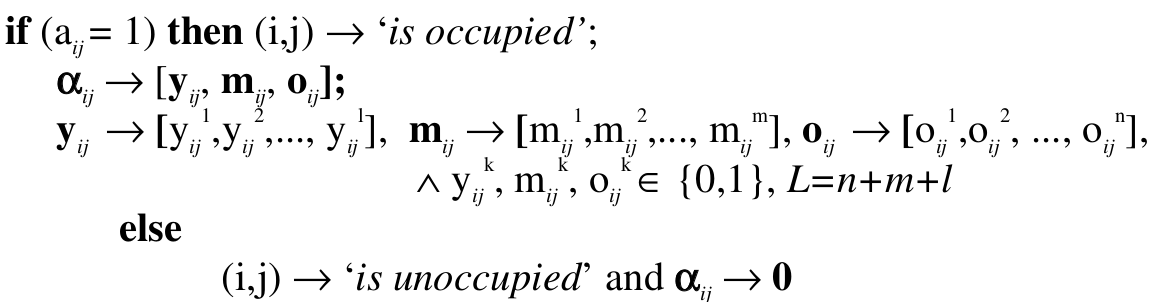
\includegraphics[width=.5\textwidth]{imagens/estrutura-alpha}
\caption{Exemplo das estrutura if-them e alpha \cite{dzwinel:04}.}
\label{fig:estrutura-alpha}
\end{figure}

Os vetores binários $\textbf{y}_{ij}$, $\textbf{m}_{ij}$, $\textbf{o}_{ij}$
representam os episódios de vida de um indivíduo: a ``juventude'', a 
``maturidade'' e a ``velhice'', respectivamente. As variáveis \textbf{l},
\textbf{m} e \textbf{n} são os tempos máximos de cada episodio de vida
enquanto que a duração atual de cada episódio é o numero de 1's em cada vetor
$\textbf{y}_{ij}$, $\textbf{m}_{ij}$, $\textbf{o}_{ij}$.

A reprodução é feita usando a vizinhança de Moore que procura os dois
primeiros vizinhos no episódio da ``maturidade'' e passa para um algorítimo
genético (ag) fazer a reprodução.

A Figura \ref{fig:pseudo-codigo-evolucao} mostra a sequência de instruções
do processo de evolução da matriz. 

\begin{figure}[ht]
\centering
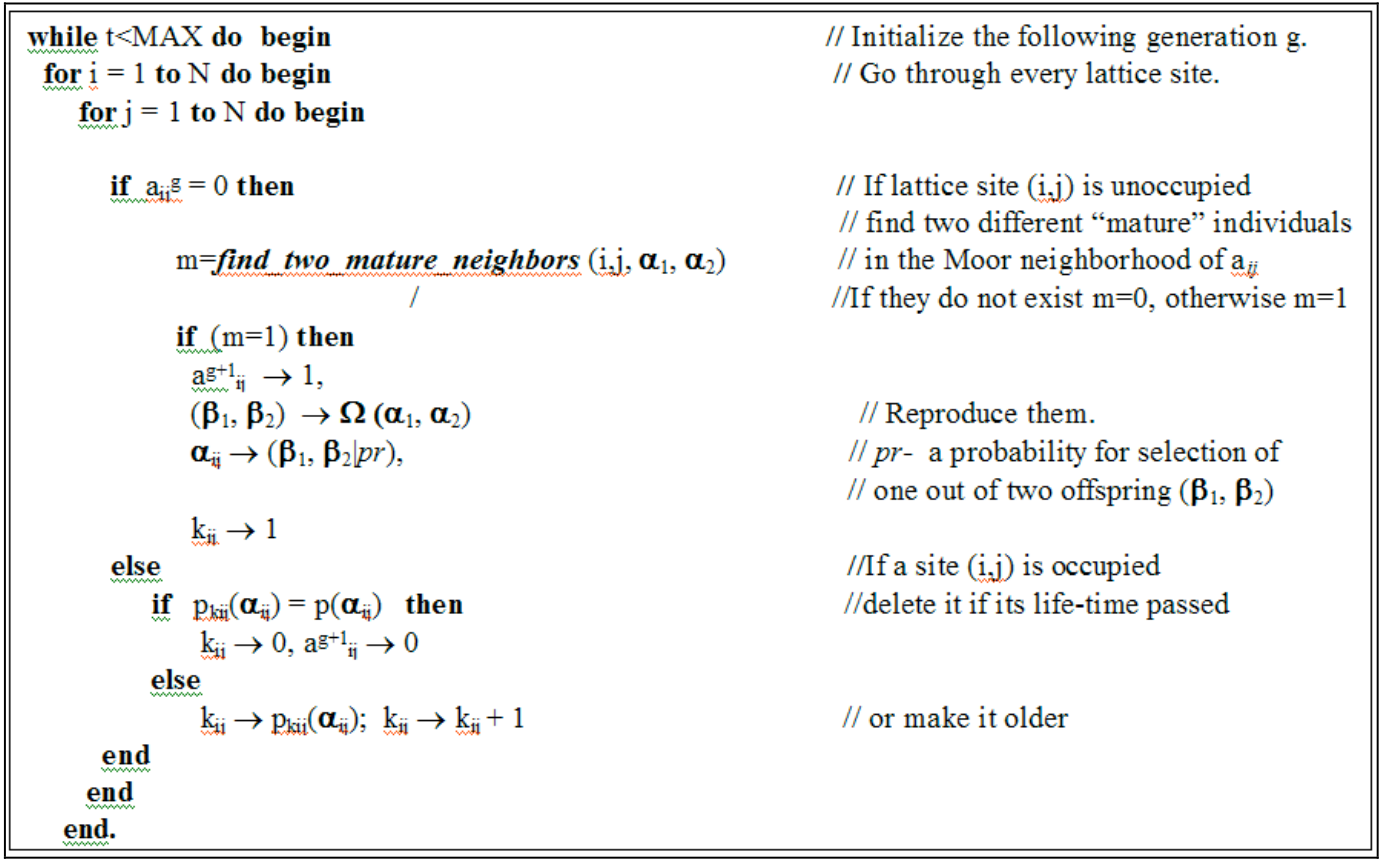
\includegraphics[width=.5\textwidth]{imagens/pseudo-codigo-evolucao.png}
\caption{Pseudo-código que descreve as regras de evolução \cite{dzwinel:04}.}
\label{fig:pseudo-codigo-evolucao}
\end{figure}

A variável \textit{t} é o número de gerações do automato celular (tempo). A
função p($\alpha _{ij}$) retorna o número de 1's do indivíduo
\textbf{$\alpha _{ij}$}. Já a função p$_{k}$($\alpha _{ij}$) é definida como
segue:

$\forall (a_{ij} = 1 \wedge p(\alpha _{ij}) \geq k); p_{k}(\alpha_{ij}) = k.$

O simbolo \textbf{$\Omega$} denota o operador de recombinação dos algoritmos
genéticos \cite{dzwinel:04}. A função \textbf{$\Omega$} não faz a mutação
genética, pois a implementação de Dzwinel tem por objetivo analisar a
influência de fatores ambientais sobre o processo de envelhecimento. Por isso
é executado apenas um \textit{cross-over} sobre os dois vizinhos selecionado e
escolhido aleatoriamente um deles.

Agora para o ambiente instável a população pode ser atacada por uma praga que
é representada por ``\textit{seeds}''. Estas sementes são jogadas na matriz do
automato celular periodicamente. Se ``\textit{seeds}'' jogada em uma área 
vazia ela movimenta-se até encontrar um indivíduo, caso contrario ambos são
eliminados da matriz. Quando uma ``\textit{seeds}'' encontra um indivíduo
ambos são eliminados da matriz. A força da praga é definida pelo
$\epsilon_{0}$ que vai ser multiplicado pela população atual e vai definir o
número de ``\textit{seeds}'' que vão ser geradas.


% ----------------------------------------------------------------------------
\section{Proposta}
%Nesta sessão tem o objetivo de explicar o trabalho proposto, ressaltando as
%contribuições da proposta.

O presente artigo tem o objetivo de fazer uma modificação na solução proposta
por Dzwinel. Para fazer a reprodução ele usa basicamente o operador de cross-
over e sorteia aleatoriamente um dos vizinhos resultante. Para este trabalho, 
para fazer a reprodução sera usado parte da técnica de \textbf{Busca Tabu}
(\textit{Tabu Search}).

A Busca Tabu é uma técnica de busca local que teve origem nos trabalhos de
Fred Glover e Pierre Hansen. De forma prática essa técnica salta de uma
solução para outra que seja seu melhor vizinho e conforme salta armazena as
melhores soluções encontradas para escapar do ótimo local.

A Figura \ref{fig:busca-tabu} mostra o processo de escolha da Busca Tabu.
Onde é selecionado uma solução aleatoriamente, no exemplo foi a célula B2 com
o avaliação igual a 90.

\begin{figure}[h!]
\centering
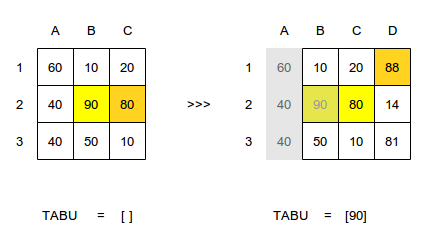
\includegraphics[width=.5\textwidth]{imagens/busca-tabu}
\caption{Exemplo do processo da Busca Tabu.}
\label{fig:busca-tabu}
\end{figure}

Inicialmente é avaliado cada vizinho e selecionado o que tem a melhor
avaliação, no exemplo foi a célula C2 com avaliação 80. Em seguida é colocado
a célula B2 na lista Tabu que é uma lista de movimentos proibidos. O processo
de avaliar a vizinhança é realizado para a célula B2, mas observando a lista
Tabu.

A lista Tabu reduz o risco do algoritmo entrar em ciclo, porem pode proibir
movimentos para uma solução que ainda não foi visitada. Para evitar isso
existe a \textbf{função de aspiração} que é a função que retira uma solução da
lista Tabu.

A Busca Tabu é interrompida quando atingir um número máximo de iterações sem
melhora na solução e quando o valor da melhor solução for menor que a menor
solução conhecida ou próxima a ela.

Os parâmetros de controle da Busca Tabu são o tamanho da lista tabu, a função
de aspiração, o número de soluções vizinhas testadas em cada iteração e o
número máximo de iterações sem melhoras na solução.

Para este trabalho foi modificada a implementação feita em \cite{dzwinel:04}
que utilizou um Algoritmo Genético, sem mutação genética, para fazer a 
reprodução dos indivíduos. A reprodução acontecia através do
\textit{cross-over} do código genético de dois vizinhos maduros gerando dois
filhos. E a escolha de qual filho seria escolhido era aleatória. Para
tentar obter resultados melhores foi modificado a forma de buscar os vizinhos,
onde agora é testado todos os vizinhos maduros e selecionado os dois melhores.
Estes são combinados usando \textit{cross-over} e ambos são avaliados para
o melhor entre eles tornar-se o indivíduo da célula testada. 


% ----------------------------------------------------------------------------
\section{Resultados Alcançados}

Se possível comparando com o trabalho referencial.

% ----------------------------------------------------------------------------
\section{Conclusões}

Apresentar as conclusões  \cite{dzwinel:04}.

%\begin{table}[ht]
%\centering
%\caption{Variables to be considered on the evaluation of interaction
%  techniques}
%\label{tab:exTable1}
%\includegraphics[width=.7\textwidth]{table.jpg}
%\end{table}

% ----------------------------------------------------------------------------

\bibliographystyle{sbc}
\bibliography{se-alexandre}

\end{document}
